\chapter{}

\titleimg{manna}

\mktitle{Capitulum Sextum Decimum}
\thispagestyle{empty}

\cstart{P}{rofectīque} sunt dē Elim, et vēnit omnis multitūdō fīliōrum
Isrāēl in dēsertum Sīn, quod est inter Elim et Sināī,
quintodecīmō diē mēnsis secundī, postquam ēgressī sunt dē terrā Ægyptī.

\vnum{2}Et \mpp{murmurāre:}{loqui de re quae non placet}murmurāvit omnis \mpp{congregātiō, -ōnis (f):}{grex hominum}congregātiō fīliōrum
Isrāēl contrā Moysēn et Aarōn in \mpp{sōlitūdo, -inis (f):}{locus ubi
nemo vel unus habitat}sōlitūdine. \vnum{3}Dīxēruntque fīliī Isrāēl ad eōs:
``Utinam mortuī essēmus per manum Dominī in terrā Ægyptī, quandō sedēbāmus
super \mimg{olla}{ōlla, -ae (f)}ōllās carnium, et \mpp{comedere:}{totum ēsse;
ēsse}comedēbāmus pānem in \mpp{saturitās, -ātis (f)}{< satis}saturitāte: cūr ēdūxistis nōs in
dēsertum istud, ut occīderētis omnem multitūdinem famē?''

\vnum{4}Dīxit autem
Dominus ad Moysēn: ``Ecce ego \mpp{pluere:}{imbrem facere}pluam vōbīs pānēs
dē cælō: ēgrediātur populus, et \mpp{colligere:}{invenīre rēs quae hīc illīc sunt, deinde sumere eās atque in unō locō ponere}colligat quæ
\mpp{sufficere:}{satis esse}sufficiunt per singulōs diēs: ut
\mpp{tentāre:}{conārī aliquid ut videatur quid fiat}tentem eum utrum ambulet in lēge meā, an nōn. \vnum{5}Dīē autem
sextō pārent quod \mpp{īnferre <}{in + ferre}īnferant: et sit \mpp{duplus/a/um:}{bis tantus}duplum
quam colligēre solēbant per singulōs diēs.''

\vnum{6}Dīxēruntque Moysēs et Aarōn ad omnēs fīliōs Isrāēl: ``Vespere sciētis
quod Dominus ēdūxerit vōs dē terrā Ægyptī, \vnum{7}et manē vidēbitis glōriam
Dominī: audīvit enim \mpp{murmur, murmuris (n):}{sonus hominis qui loquitur de re quae non placet}murmur vestrum contrā Dominum: nōs
vērō quid sumus, quia \mpp{mussitāre:}{parvā voce dicere}mussitāstis contrā nōs?''

\vnum{8}Et ait Moysēs: ``Dabit vōbīs Dominus vespere carnēs edere, et manē pānēs in
saturitāte: eō quod audierit \mpp{murmurātio, -ōnis (f) <}{murmurāre}murmurātiōnēs
vestrās quibus murmurātī estis contrā eum: nōs enim
quid sumus? Nec contrā nōs est murmur vestrum, sed contrā Dominum.''

\vnum{9}Dīxit quoque Moysēs ad Aarōn: ``Dīc ūniversæ \mpp{congregātiō, -ōnis (f):}{grex hominum}congregātiōnī
fīliōrum Isrāēl: Accēdite cōram Dominō: audīvit enim murmur vestrum.''

\vnum{10}Cumque loquerētur Aarōn ad omnem \mpp{cœtus, -ūs (m):}{congregātiō}cœtum fīliōrum Isrāēl, \mpp{respicere:}{aspicere iuvandī
causā}respexērunt ad sōlitūdinem: et ecce glōria Dominī appāruit in nūbe.

\vnum{11}Locūtus est autem Dominus ad Moysen, dīcēns: \vnum{12}``Audīvī murmurātiōnēs
fīliōrum Isrāēl. Loquere ad eōs: Vespere comedētis carnēs, et manē
\mpp{saturāre:}{tam multum ēsse ut fortasse dicas ``bene, bene, satis est!''}saturābiminī pānibus: sciētisque quod ego sum Dominus Deus
vester.''

\begin{figure}[h!]
    \begin{minipage}[hp]{0.5\linewidth}
        \centering
        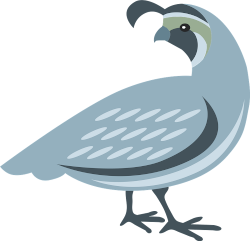
\includegraphics{quail}
        \caption{coturnīx, -īcis (f)}
    \end{minipage}%
    \begin{minipage}[hp]{0.5\linewidth}
        \centering
        
\includegraphics{dew}
        \caption{rōs, rōris (m)}
    \end{minipage}
\end{figure}

\vnum{13}Factum est ergō vespere, et ascendēns coturnīx
\mpp{cooperīre:}{operīre}cooperuit \mpp{coturnīx cooperuit castra:}{coturnīcēs cooperuērunt castra}castra: manē 
quoque rōs iacuit per \mpp{circuitus, -ūs (m):}{locus circum alterum
locum}circuitum castrōrum. \vnum{14}Cumque operuisset \mpp{superficiēs, -eī (f):}{summa pars reī quae operit aliās īnferiorēs partēs}superficiem
terræ, appāruit in
sōlitūdine \mpp{minūtus/a/um:}{parvus}minūtum, et quasi \mpp{pilum, -ī (n):}{baculum minimum quō homo herbās aliāsque rēs frangit in parvō poculō} pilō \mpp{tūsus/a/um:}{pulsatus}tūsum in
\mpp{in similitūdinem pruīnae:}{similis pruīnae}similitūdinem \mpp{pruīna, -ae (f):}{rōs frigidissimus}pruīnæ super terram. \vnum{15}Quod
cum vīdissent fīliī Isrāēl, dīxērunt ad \mpp{ad invicem:}{inter sē}invicem: ``Manhu?'' quod significat: ``Quid est
hoc?'' Ignōrābant enim quid esset. 

Quibus ait Moysēs: ``Iste est pānis quem
Dominus dēdit vōbīs ad \mpp{vēscī:}{ēsse}vēscendum. \vnum{16}Hic est sermō, quem
\mpp{praecipere:}{imperāre}præcēpit Dominus: Colligat ūnusquisque ex eō
quantum sufficit ad vēscendum: \mpp{gomor:}{mensura Hebraeōrum}gomor per singula capita,
iuxtā numerum animārum vestrārum quæ habitant in
\mimg{tab2}{tabernāculum, -ī (n)}tabernāculō sīc tollētis.''

\vnum{17}Fēcēruntque ita fīliī Isrāēl:
et collēgērunt, alius plūs, alius minus. \vnum{18}\mpp{mētior, mētīrī, mēnsus sum:}{e.g, homo habet magnum vas aquae plenum et oportet eum fundere aquam in decem alia parva vasa. Dicimus hominem mētīrī aquam}Et mēnsī sunt
ad \mpp{mēnsūra, -ae (f):}{e.g, ``da mihi decem vasa aquae plena!'' Vas dicitur mēnsūra aquae}
mēnsūram gomor: nec quī plūs collēgerat, habuit
\mpp{amplius =}{plus}amplius: nec quī minus parāverat, reperit minus: sed
singulī iuxtā id quod edere poterant, \mpp{congregāre:}{in unum locum
cōgere vel ferre vel ducere}congregāvērunt. 

\vnum{19}Dīxitque Moysēs ad eōs: ``Nūllus relinquat ex eō in manē.''

\vnum{20}Quī nōn audiērunt eum, sed
dīmīsērunt quīdam ex eīs usque manē, et \mimg{vermis}{vermis, -is (m)}\mpp{scatēre:}{plēnum esse}scatēre cœpit
vermibus, atque \mpp{computrēscere:}{facere malum odorem
(id quod nasus sentit) propter rem mortuam}computruit: et īrātus est
contrā eōs Moysēs. \vnum{21}Colligēbant autem māne singulī,
quantum sufficere poterat ad vēscendum: cumque \mpp{incalesco, incalescere, incaluī:}{valde calidus fiērī}incaluisset
sōl, \mpp{liquefiērī:}{fiērī res fluens sicut aqua}liquefiēbat. \vnum{22}In diē autem sextā collēgērunt cibōs
\mpp{duplex, duplicis (adj):}{bis tantus}duplicēs, id est, duo gomor per singulōs hominēs: vēnērunt
autem omnēs prīncipēs multitūdinis, et nārrāvērunt Moȳsī. 

\vnum{23}Quī ait eīs:
``Hoc est quod locūtus est Dominus: \mpp{requiēs, requiēī (f):}{tempus quo homo non
laborat}Requiēs \mpp{sabbatum, -ī (n):}{dies septimus quō non licet hominibus laborāre}sabbatī \mpp{sānctificāre:}{sanctum
facere}sānctificāta est Dominō crās: quodcumque operandum est, facite, et
quæ coquenda sunt coquite: quidquid autem reliquum fuerit, repōnite usque
in manē.''

\vnum{24}Fēcēruntque ita ut præcēperat Moysēs, et nōn computruit, neque
vermis inventus est in eō.

\vnum{25}Dīxitque Moysēs: ``Comedite
illud hodiē, quia sabbatum est Dominī: nōn inveniētur
hodiē in agrō. \vnum{26}Sex diēbus colligite: in diē autem
septimō sabbatum est Dominī, \mpp{idcircō:}{proptereā, ideō}idcircō nōn
inveniētur.''

\vnum{27}Venitque septima diēs: et ēgressī dē populō ut
colligerent, nōn invēnērunt.

\vnum{28}Dīxit autem Dominus ad
Moysēn: ``\mpp{usquequō:}{usque ad quod tempus?}Us\-quequō nōn vultis
cūstōdīre \mpp{mandātum, -ī (n):}{id quod imperatum vel traditum
est}mandāta mea et lēgem meam? \vnum{29}Vidēte quod Dominus dederit vōbīs
sabbatum, et propter hoc diē sextā \mpp{tribuere:}{dāre}tribuit vōbīs cibōs
duplicēs: maneat ūnusquisque apud \mpp{sēmetipsum =}{sē}sēmetipsum; nūllus
ēgrediātur dē locō suō diē septimō.''

\vnum{30}Et \mpp{sabbatīzāre:}{sabbatum colere}sabbatīzāvit
populus diē septimō. \linebreak\vnum{31}Appellāvitque domus Isrāēl nōmen eius Mān: quod erat quasi sēmen
\mpp{coriandrum, -ī (n):}{quaedam herba}coriandrī album, \mpp{gustus, -ūs (m) < gustāre}{}gustusque eius quasi
similæ cum melle.

\vnum{32}Dīxit autem Moysēs: ``Iste est sermō, quem præcēpit
Dominus: Implē gomor ex eō, et cūstōdiātur in futūrās
retrō \mpp{generātio, -ōnis (f):}{e.g una generatio
parentibus constat, līberīs eōrum altera generatio constat,
etc...}generātiōnēs: ut nōverint pānem, quō aluī vōs in sōlitūdine, quandō
ēductī estis dē terrā Ægyptī.''

\vnum{33}Dīxitque Moysēs ad Aarōn: ``Sūme vās ūnum,
et mitte ibi mān, quantum potest capere gomor, et repōne cōram Dominō ad
servandum in generātiōnēs vestrās, \vnum{34}sīcut præcēpit Dominus Moȳsī.''

Posuitque illud Aarōn in tabernāculō reservandum. \vnum{35}Fīliī autem Isrāēl
comēdērunt mān quadrāgintā annīs, dōnec venīrent in terram \mpp{habitābilis, -e (adj):}{habitārī potest}habitābilem: hōc cibō alitī sunt, usquequō
tangerent fīnēs terræ Chanaan.

\vnum{36}Gomor autem decima pars
est \mpp{ephī (n) (indec):}{mensura Hebraeōrum}ephī.
